
\documentclass[12pt,oneside,a4paper]{article}

\usepackage[svgnames]{xcolor}

\usepackage{amsmath}

\usepackage{wallpaper}

\usepackage{tikz}

\usepackage[section]{placeins}

\usepackage[
    top=2.5cm,
    bottom=2.5cm,
    left=4cm,
    right=2.5cm
]{geometry}

\ifdefined\DEBUG
    \usepackage{showframe}
\fi

%\renewcommand{\familydefault}{\sfdefault}
\usepackage[utf8]{inputenc}

\usepackage[english]{babel}
\usepackage{csquotes}

\usepackage{graphicx}

\usepackage[round]{natbib}

\usepackage{setspace}
\onehalfspacing

\usepackage[ddmmyyyy]{datetime}
\renewcommand{\dateseparator}{.}
%\newdate{date}{06}{07}{2015}
%\date{\displaydate{date}}

\ifdefined\PRINT
    \usepackage[hidelinks]{hyperref}
\else
    \usepackage{hyperref}
\fi

\usepackage[xindy]{glossaries}


\newglossaryentry{abstract factory}{
    name={abstract factory},
    description={\citeauthor{gamma:1993} describe a design pattern in their book "Design Patterns" that can be applied to this problem.
    An abstract factory helps "creating families of related or dependent objects without specifying their concrete class"\citep[p.~99]{gamma:1993}.}
}

\newglossaryentry{amazon.com}{
    name={Amazon.com},
    description={One of the biggest internet based retailers in the world with focus electronic commerce and cloud computing.}
}

\newglossaryentry{dynamic programming}{
    name={dynamic programming},
    description={\color{red}TODO}
}

\newglossaryentry{e-commerce}{
    name={e-commerce},
    description={{\color{red}TODO}}
}

\newglossaryentry{eBay}{
    name={eBay},
    description={{\color{red}TODO}}
}

\newglossaryentry{rs}{
    name={RS},
    description={Abbreviation for recommender systems.}
}

\newglossaryentry{git}{
    name={git},
    description={\color{red}TODO}
}

\newglossaryentry{ir}{
    name={IR},
    description={Abbreviation for information retrieval.}
}

\newglossaryentry{nodejs}{
    name={node.js},
    description={\color{red}TODO}
}

\newglossaryentry{python}{
    name=Python,
    description={
        A widely used scripting language with focus on readable source-code.
    }
}

\newglossaryentry{pybottle}{
    name=bottle,
    description={
        A python based web-framework that supports routing, templates and contains a web-server.
    }
}

\newglossaryentry{sqlite3}{
    name=SQLite3,
    description={
        A relational database system with support of Transactions and Views. It is also included in one of the standard Python-modules.
    }
}

\newglossaryentry{sphinx}{
    name=Sphinx,
    description={
        A document generator initially built for Python. It creates a documentation from docstrings within the Python source code.
    }
}

\newglossaryentry{web api}{
    name={web API},
    description={\color{red}TODO}
}

\newglossaryentry{zalando}{
    name={Zalando},
    description={A online shop specialized on clothing}
}


\begin{document}

% titlepage


\newcommand{\TitleHRule}{\rule{\linewidth}{0.5mm}}

\LRCornerWallPaper{0.5}{./inc/titlepage/fau-watermark-seal}

\begin{titlepage}


    \begin{center}

    { \huge \bfseries Clothing recommendation based on Rocchio's algorithm\\[0.4cm]}
    \bigskip
    { \huge Design and prototypical implementation}
    
    %\vfill
    {\vspace{3cm}}
    %{\vspace{6cm}}

    %{\vspace{3cm}}

        Zwischenbericht zur\\
        \textbf{Bachelorarbeit}\\
        an der Friedrich-Alexander Universit\"at Erlangen-N\"urnberg\\
        {\vspace{1cm}}
        %
\includegraphics[width=70mm]{./inc/titlepage/fau-logo}
        
\includegraphics[width=\textwidth/4*3]{./inc/titlepage/fau-logo}


    \vfill
    \TitleHRule

    \begin{tabular}{ r l }
        Eingereicht von:    & \myAuthor\\
                            & \myStreet\ \myNumber\\
                            & \myPlz\ \myCityPartOne\"u\myCityPartTwo\\
        Matrikelnummer:     & \myMatrnr\\
        Studiengang:        & \myCourse\\
        Referent:           & \myProf\\
        Betreuer:           & \myTutor 
    \end{tabular}

    \TitleHRule

    \end{center}

\end{titlepage}

\ClearWallPaper






% Table of content
\tableofcontents
\clearpage

% the text

\section{Introduction}

% Choice overload
% Aktuelle Situation in der Kleidungsbranche
% kurzer Einblick in Recommender systems (wird spaeter weiter ausgefuehrt)


When a typical customer enters a shop or department store, he often gets confronted with a very large amount of products he can choose from.
This is especially true, when searching for products on the internet in a web shop.
The commonly known web shop amazon.com for instance offers about 280 million different products on their internet presence for the United States.\citep{marketplaceanalytics:2014}
Even shops dedicated to only a special kind of product have a wide array of products.
On Zalando, a German online shop dedicated to clothing, one can choose out of 150.000 products of 1.500 different brands.\citep{visser:2014}\\
There is a general belief that great choice pleases the customers needs.
However it is actually proven, that this idea is not fully correct and reality is much more complex.
Already in 2000 a group of scientists demonstrated, that a great variety can also have negative effects.\citep[312]{diehl:2010}
It is proven, that large assortments can lower the customers willingness to purchase products.\citep[313]{diehl:2010}
Furthermore to much choice can also lower the customers satisfaction.\citep[320]{diehl:2010}


Since especially online-shops have a overwhelming great assortment of products, they struggle most with the problem of overloading their potential customers with products.
Therefore many online shops have already implemented recommendation systems to aid their customers by finding the right product.
Most modern recommender engines give for every user customized recommendations - these ones are also called personalized recommendation system.
But early versions also gave static recommendations that were the same for every user.\citep[1-2]{ricci:2011}




There are different possible approaches to recommendation systems and some of them will be discussed in the later sections of this thesis.






% personal vs. non-personal RS






\section{Recommender systems}
%%%%%%%%%%%%%%%%%%%%%%%%%%%%%%%%%%%%
\iffalse Aufgaben eines Recommender systems \fi
%%%%%%%%%%%%%%%%%%%%%%%%%%%%%%%%%%%%
Even though has already been a brief introduction into recommender systems a much more in depth view will follow.
When describing a RS, one also has to describe the different users and the goal they want to achieve.
On the one hand is the provider of an RS.
Let's assume that the provider is a huge online shop selling apparel.
On the other hand, there is the client using the RS to find products best suited for his needs.
In case of a online shop the user probably wants clothing that is after his fancy and in his size.
The online shop however, pursues many more objectives.
When he offers a RS to the user, he wants to
\begin{itemize}
    \item\textbf{Increase sells}\hfill\\
        By determining and offering the items the user likes most, the chance of the user buying the praised product will grow.
    \item\textbf{Selling more diverse items}\hfill\\
        Often the user only has a vague idea of the product he wants and only knows the well-established ones.
        RS can help to recommend products he wouldn't find otherwise.
    \item\textbf{Increase user satisfaction to gain customer loyalty}\hfill\\
        With good recommendations and a pleasing user interface the user is more likely to accept recommendations.
    \item\textbf{Increase user fidelity}\hfill\\
        A RS links the using behaviour to the users previous one.
        This helps to get a more accurate picture of the users preferences.
    \item\textbf{Gain better understanding about the users needs}\hfill\\
        When the general preferences of users are known, it is possible to adapt the internal work flow of the RS provider to the user.
        This means, that an apparel shop can increase the stock on some specific cuts/patterns or colours, since the customers will demand them.
\end{itemize}
as mentioned by \citeauthor[p.~4-5]{ricci:2011}.\\
So there are various reasons for online service provider to introduce RS as an additional service to support their business.

\subsection{Data and knowledge sources}
\label{sec:dataknowledgesource}
Any RS needs data from which the suggested items will be calculated and most of the time information about the requesting user is also necessary.
The data heavily influences the selection of recommender algorithms which provide suggestions for the user.\citep[p.~7-8]{ricci:2011}
%There are knowledge poor algorithms whose input data solely consists of user rankings.
%But there also so called knowledge dependent algorithms using social relationship or activities of users for instance.\citep[p.~7-8]{ricci:2011}
Any resource a recommender can use is classified as either an item, a user, or a transaction.

\paragraph{Item}~\\
Items are the products that will be suggested to the user.
In the case of an apparel shop this will be clothing and maybe some products that are related such as handbags or accessoire like sunglasses, etc.
For any item a complexity can be estimated.
There are factors such as its structure, textual representation, as well as time dependent importance of a product.
Even thought clothing may contain certain time-dependency (winter vs. summer season), its general complexity is rather low.
A typical high complexity item may be insurence policies, jobs, or financial investments.
Items can also be distinguished by their value and its costs.
While the value states how valueable the item is for the user, costs are the combination of monetary value of the item plus the effort to require information about and getting it.
With the complexity of a product rising, also the effort to inform oneself about it will increase.
\citep[p.~8]{ricci:2011}

\paragraph{User}~\\
All users differ from each other - therefore one can not simply make a recommendation which satisfies every users needs.
In order to generate a matching recommendation for a given user information about him or his preferences are necessary.
Diverse recommendation approaches use different kinds of data.
These different ways will be discussed later, in section~\ref{sec:recommenderapproaches}.
The data, however, one can collect about the user is manifold.
It ranges from demographic information such as age, size, sex, nationality/cultural background, income to his behaviour as shown in search queries or ratings for a specific kind of product.
Any of the named attributes is relevant for an online clothing store, as they determine the brand (possibly influenced by income), imprint (may depend on age), and so on.\citep[p.8-9]{ricci:2011}
It is also possible, to use item-rankings or purchase history provided by users to compare the similarity of users.\citep[p.~377-378]{pradel:2011}

\paragraph{Transactions}~\\
\label{sec:feedback}
Transaction describe the interaction between the user and the RS.\citep[p.~9]{ricci:2011}
It can be differentiated into explicit and implicit feedback from the user towards the RS.
While explicit feedback requires the users to evaluate certain items in order to get a picture of the users preferences, implicit doesn't.
Instead implicit feedback will be gained by monitoring the user.\citep[p.~76-77]{lops:2011}
So implicit feedback will be provided by the normal usage of the online shop.
This means, that every time the user interacts with a product, i.g. by viewing it, the RS learns that this product may be relevant to the user.\citep{taghipour:2007}
The interaction with the RS includes the users browsing patterns (in a web based RS), his search queries and can also involve the users mouse movement (when he uses a computer).\citep[p.~146]{koren:2011}
A online clothing store could for example use the clients search queries, how long he views a specific product.\\
In contrary explicit feedback needs the users active involvement.
The most common sources for explicit feedback are a rating wheter the user likes the product or not, or a textual comment - also describing, wheter he likes it nor not.
The attitude towards a product will often be retrieved through a rating.
Common ones are either binary ratings with like and dislike as possible values, or some where the user can rate a product with points, similiar to grades.\citep[p.~77]{lops:2011}


TODO

Erkl"aren abgrenzung zwischen knowledge und context


\subsection{Different approaches}
\label{sec:recommenderapproaches}
%%%%%%%%%%%%%%%%%%%%%%%%%%%%%%%%%%%%
\iffalse
was fuer welche gibt es
wie unterscheiden sie sich
\fi
%%%%%%%%%%%%%%%%%%%%%%%%%%%%%%%%%%%%
As already mentioned there are various sources of information a recommender system can use and the choice heavily impacts the quality of recommendations.
Different algorithms are suited for different tasks and have some drawbacks.\citep[p.~377-378]{burke:2007}
As knowledge has already been introducted in section~\ref{sec:dataknowledgesource} we will further focus on them.
There are four major approaches which we will discuss and adapt to the example of an online clothing shop.

\paragraph{Content-based}~\\
Each item is defined by its attributes such as its colour, price, age, etc.
And each user has his own rating for each of the attributes which determine whether he likes the item or not.
Every time the user gives feedback to the RS in form of preferencing or rejecting an item the RS will adapt its information about the users preferences of the items attributes.
The RS determines items it can recommend to the user by comparing each of the items attributes with the users preference.
\citep[p.~75]{lops:2011}\\
In reference to a clothing store every product can be defined through its colour, brand, price, pattern and so on.
Every user however, has his very own rating for each of the attributes.
The closer all attributes of an item match the preference of a user, the higher is the probability that the user likes the item.
A content-based approach will be implemented and further described in section~\ref{sec:implementation-contentbased}.
As recommender algorithm Rocchio's algorithm will be used (section~\ref{sec:rocchio}).

\paragraph{Collaborative filtering}~\\
The idea of collaborative filtering is based on similarity of users.
Two Users which are similiar in their preferences are more likely to predict useful items for each other.
In order to determine which users have similiar opinions towards the items, their item-ratings are beeing compared.
\citep[p.~291-292]{schafer:2007}
Within an online clothing store this can be achieved by introducing a rating system for clothing.
When all users give their opinion about the clothes for every user a matching partner can be found.
Assuming that there are two user (user $A$ and user $B$) with similiar preferences, preferenced clothings from $A$ can be suggested to $B$ if $B$ hasn't evaluated the piece of clothing yet.

\paragraph{Demographic}~\\
These systems rely on demographic data which is available for every user.
Assumptions about user preferences are build upon the assumption, that the users demographic profiles provides enough information to estimate his preferences.
Demographic data can consist of the users age, sex, nationality/cultural background, income, etc.\citep[p.~12]{ricci:2011}
Income for instance can give information whether clothing of well-known brands is appropriate or not.

\paragraph{Knowledge-based}~\\
Knowledge-based approaches rely on domain-knowledge about items and need additional information about the users needs.
\citep[p.~12-13]{ricci:2011}

TODO

Knowledge based besser erkl\"aren

\begin{figure}[h]
    \center
    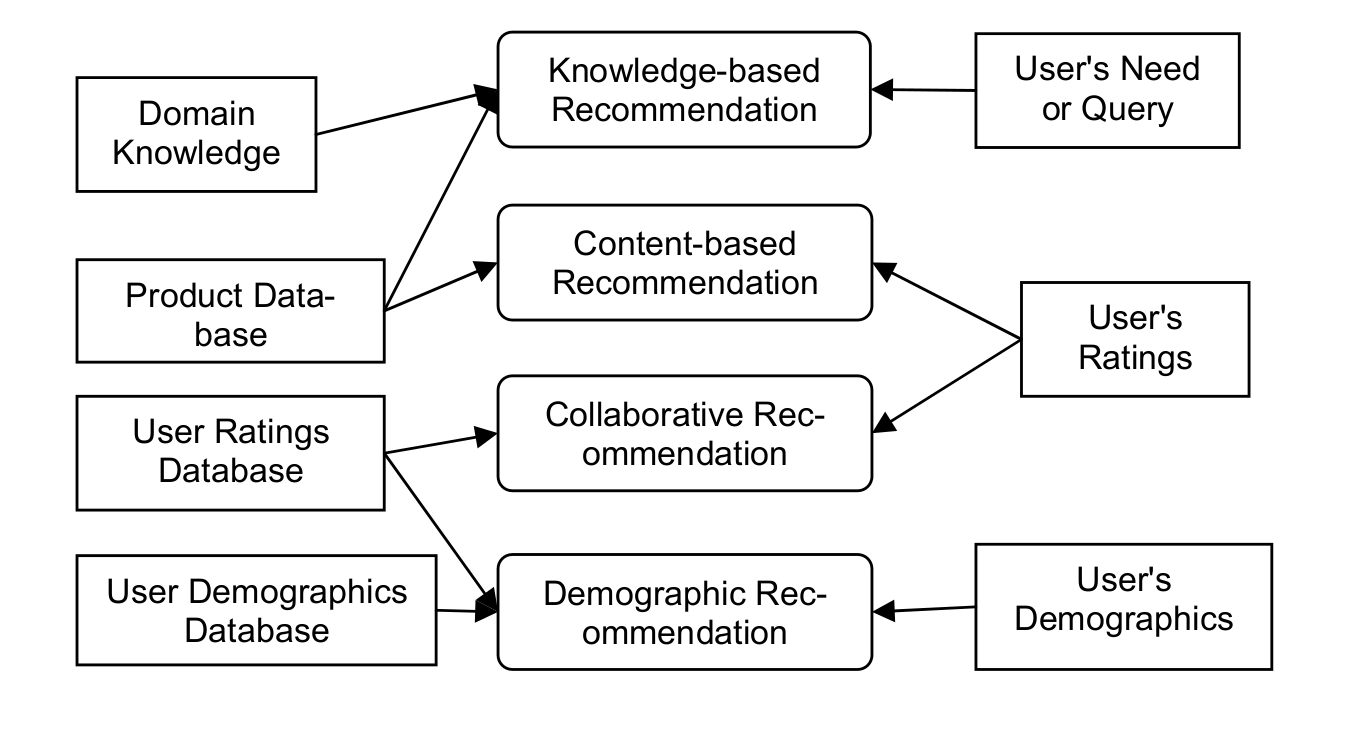
\includegraphics[scale=0.3]{inc/recommendersystems/RecommendationTechniquesAndKnowledgeSources.png}
    \caption{Recommendation techniques and their knowledge sources.\citep[p.~379]{burke:2007}}
\end{figure}

\subsection{Comparison}
%%%%%%%%%%%%%%%%%%%%%%%%%%%%%%%%%%%%
vor- und nachteile
\"Ubersicht \"uber alle System (fancy Tabelle?)
%%%%%%%%%%%%%%%%%%%%%%%%%%%%%%%%%%%%

\subsection{Mixing different RS approaches together}
%%%%%%%%%%%%%%%%%%%%%%%%%%%%%%%%%%%%
\iffalse
Hybrid web recommender systems
\fi
%%%%%%%%%%%%%%%%%%%%%%%%%%%%%%%%%%%%

\subsection{Critics on RS}
%%%%%%%%%%%%%%%%%%%%%%%%%%%%%%%%%%%%
Bei Onlinezeitungen: Nutzer bekommen nur noch Artikel die sie lesen wollen --> verdummung?
%%%%%%%%%%%%%%%%%%%%%%%%%%%%%%%%%%%%


\section{Information retrieval}
%%%%%%%%%%%%%%%%%%%%%%%%%%%%%%%%%
\iffalse
Was ist Information retrieval
in depth implementation is out of scope
Hinleitung zu Vektoren
\fi
%%%%%%%%%%%%%%%%%%%%%%%%%%%%%%%%%
\citeauthor{manning:2009} describe Information Retrieval in their book as process of "finding material [\ldots] of an unstructured nature [\ldots] that satisfies an information need from within a large collection."\citep[p.~1]{manning:2009}\\
In generall IR and RS are very similiar and a few technologies and findings of IR can be transfered to RS.
Since IR systems are build to handle unstructured data and transform them into a form that is easier to handle for computer systems one can adopt the method to RS input data such as items.\citep[p.~21-23]{ricci:2011}
There are various ways IR systems interpret data.
However this thesis will focus on one common method (and the theorie it depends on) called "tf-idf-vectors" which is a requirement for the Rocchio algorithm.\citep[p.~93]{lops:2011}\\
IR systems are built to handle "unstructured data".
Unstructured data is information bundled within a document (document is the IR related term for what is understood as item by RS) without any clear semantical structure.\citep[p.~1-3]{manning:2009}
The data within a document
IR systems can extract all relevant terms from a document
A term may resemble an attribute of an item such as its colour or brand.
The way of retrieving terms from a unstructured document is out of scope for this thesis but there is a brief example in figure~\ref{fig:TermRetrieving}.\\
For the section Information Retrieval the IR vocabulary will be adopted.
This means, that items will be called documents and attributes will be known as terms.

\begin{figure}[h]
    \center
    \lstset{style=customHTML}
    \begin{lstlisting}
<html>
    <head><title>Online shop</title></head>
    <body>
        <img src="/img/p_42.jpg" alt="FancyBrand's product"/>
        <table>
            <tr><td>Colour</td><td>green</td></tr>
            <tr><td>Price</td><td>24,95 &euro;</td></tr>
            <tr><td>Brand</td><td>FancyBrand</td></tr>
        </table>
    </body>
</html>
    \end{lstlisting}
    \begin{tabular}{ l }
        \textbf{Terms:}\\\hline
        green\\
        24,95 \&euro;\\
        FancyBrand%\\\hline
    \end{tabular}
    \caption{Retrieving Terms from a HTML document.}
    \label{fig:TermRetrieving}
\end{figure}


\subsection{Weighting}
As already mentioned a document can be be described as a collection of terms.
The process of locating terms within a document is taken for granted.
When a user queries for a specific term one has to find each relevant document including this term.
Also an order regarding the documents significance will be required.
The terms significance within a document is defined by its weight.\citep[p.~117]{manning:2009}\\
While primitive IR methods such as boolean retrieval only check for the existance of a queried term within a document weighting can give more precise results regarding the terms significance in a document.\citep[p.~109]{manning:2009}

\subsubsection{Term frequency}
A simple method to quantify the importance of a term within a document is the so called term frequency.
The concept is based on the assumption that the frequency of a term $t$ indicates its importance within a document $d$.
It is denoted as $\text{tf}_{t,d}$ where $t$ resembles the term an $d$ the document.
The number of occurences of $t$ within $d$ can be directly interpreted its term frequency.\citep[p.~117]{manning:2009}\\
For products of an online shop and its resulting term frequency may look like as described in figure~\ref{fig:tfweighting}.\\
\begin{figure}[h]

    Document $\text{d}1$ with identified terms underlined:\\
    \underline{blouse} \underline{blue} \underline{55} Euro. \underline{55} cm by size \underline{S}. 100\% \underline{Polyester}

    \center
    \vspace{5mm}
    \rowcolors{0}{\dustRowColourFirst}{\dustRowColourSecond}
    \begin{tabular}{ l l }
        \rowcolor{\dustRowColourHead}
        \multicolumn{2}{c}{Term frequency}\\\hline
        $\text{tf}_{\text{blouse},\text{d1}}$       & 1\\
        $\text{tf}_{\text{blue},\text{d1}}$         & 1\\
        $\text{tf}_{\text{55},\text{d1}}$           & 2\\
        $\text{tf}_{\text{S},\text{d1}}$            & 1\\
        $\text{tf}_{\text{Polyester},\text{d1}}$    & 1\\
    \end{tabular}

    \caption{Term frequency weighting}
    \label{fig:tfweighting}
\end{figure}

\subsubsection{Inverse document frequency}
In some domains special terms will often appear multiple times within a document and therefore have high term frequency weight without giving any explanatory value.\citep[p.~117]{manning:2009}
Documents resembling clothing offered by an online shop may always include the name of the store as term.
Since the user already explicitely searches on the store, the relevance of this term is rather low.
In order to transfer this to weighting, inverse document weighting (idf) has been implemented.
Idf will scale down the weighting of terms that appear in all documents.
To do so, an intermediate step is neccessary. Before calculating the idf for a term one has to determine both the terms document frequency ($\text{df}_t$) and the total count of documents (as $N$).
Next the idf can be calculated with following forumla:\citep[p.~117-118]{manning:2009}\\
\begin{equation}
    \text{idf}_{t} = \log\frac{N}{\text{df}_{t}}
\end{equation}
The logarithms basis isn't of great importance.\citep[p.~118]{manning:2009}
The examples however use 10 as base.
A more explanatory example is presented by figure~\ref{fig:idfweighting}.
The example states that rare items posses a higher idf, whereas more frequent terms are rated lower.\citep[p.~118]{manning:2009}\\
\begin{figure}[h]

    Total count of documents  $N$ is 500\\
    Term1 "FancyShop" appears in 500 documents\\
    Term2 "blouse" appears in 130 documents\\

    \center
    \begin{tabular}{ l | l }
        $\text{df}_{\text{FancyShop}} = 500$                                                                    & $\text{df}_{\text{blouse}} = 130$\\
        $\text{idf}_{\text{FancyShop}} = \log\frac{N}{\text{df}_{\text{FancyShop}}} = \log\frac{500}{500} = 0$  & $\text{idf}_{\text{blouse}} = \log\frac{N}{\text{df}_{\text{blouse}}} = \log\frac{500}{130} \approx 0.59$
    \end{tabular}

    \caption{Inverse document frequency weighting}
    \label{fig:idfweighting}
\end{figure}

\subsubsection{Tf-Idf}
\label{sec:tfidf}
Both the term frequency, as well as the inverse document frequency have some drawbacks.
While term frequency may weight terms with little informative value high because they appear often, inverse document frequency can totally ignore them by weighting them extremely low.
But it's possible to combine td and idf in order to get better weightings.
The result is called tf-idf.\citep[p.~118-119]{manning:2009}
\begin{equation}
    \text{tf-idf}_{\text{t,d}} = \text{tf}_\text{t,d} \times \text{idf}_\text{d}
\end{equation}

\noindent
Figure~\ref{fig:tfidfweighting} illustrates the generation of an tf-idf weighting.
\begin{figure}[h]

    Total number of documents $N$ is 3\\

    \center
    \begin{tabular}{ l l | l l l l }
        \rowcolor{\dustRowColourHead}
        Term                    & Document          & tf    & df& idf   & tf-idf\\\hline
        \multirow{3}{*}{blouse} & $\text{doc}_1$    & 15    &  \multirow{3}{*}{2}   & \multirow{3}{*}{0.18}     & 2.7\\
                                & $\text{doc}_2$    & 5     &                       &                           & 0.9\\
                                & $\text{doc}_3$    & 9     &                       &                           & 1.62\\
    \end{tabular}
    \caption{tf-idf weighting}
    \label{fig:tfidfweighting}
\end{figure}

\noindent
\citeauthor{manning:2009} describes tf-idf weighting as follows:\\
"$\text{[T]f-idf}_{\text{t,d}}$ assigns to term $t$ a weight in document $d$ that is
\begin{enumerate}
    \item highest when $t$ occurs many times within a small number of documents
    (thus lending high discriminating power to those documents);
    \item lower when the term occurs fewer times in a document, or occurs in many
    documents (thus offering a less pronounced relevance signal);
    \item lowest when the term occurs in virtually all documents."
\end{enumerate}
\citep[p.~119]{manning:2009}

\subsection{Vector space model}
\label{sec:vectorspacemodel}
Any document can now be described as a vector.
Each term in a document will be directly interpreted as component of a vector.
If a term is non existent in a document, the vector component will be numeric zero.\citep[p.~120]{manning:2009}\\
Therefore IR provids methods to describe documents as vectors.
Forging a bridge back to RS the vectors can help to provide a computer representation of real world products.
The vectors of all products can be displayed in one common vector space.
This process is known as vector space model.\citep[p.~120]{manning:2009}
An example of a two dimensional vector space model is given in figure~\ref{fig:vectorspacemodel}


\begin{figure}[h]

    \begin{quote}
        There are three documents with following terms:\\
        Document $\text{d}_1$: $1\times \text{FancyBrand}, 2\times \text{green}$\\
        Document $\text{d}_2$: $1\times \text{FancyBrand}$\\
        Document $\text{d}_3$: $1\times \text{green}$\\
        Whereas "FancyBrand" and "green" are the document terms.

        \noindent
        The generic tf-idf vector representation of one of the documents above will be:\\
        $\vec{v}_{\text{generic}} = (\text{tf-idf}_{\text{FancyBrand},\text{d}_\text{generic}}, \text{tf-idf}_{\text{green},\text{d}_\text{generic}})^T$ \\
        The corresponding tf-idf-vectors of the are:\\
        $\vec{v}_1 = (\text{tf-idf}_{\text{FancyBrand},\text{d}_1}, \text{tf-idf}_{\text{green},\text{d}_1})^T = (0.18, 0.35)^T$\\
        $\vec{v}_2 = (\text{tf-idf}_{\text{FancyBrand},\text{d}_2}, \text{tf-idf}_{\text{green},\text{d}_2})^T = (0.18, 0)^T$\\
        $\vec{v}_3 = (\text{tf-idf}_{\text{FancyBrand},\text{d}_3}, \text{tf-idf}_{\text{green},\text{d}_3})^T = (0, 0.18)^T$\\
    \end{quote}

    \center
    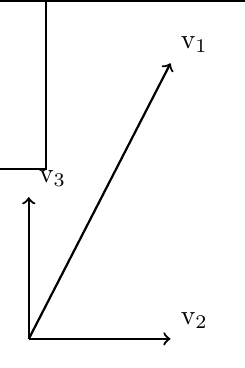
\begin{tikzpicture}
        \tkzInit[xmax=0.5,ymax=0.5,xstep=0.1,ystep=0.1]
        %\tkzAxeX[label=FancyBrand,above left=10pt]
        \tkzAxeX[label=FancyBrand, right]
        %\tkzAxeY[label=green,below right=30pt]
        \tkzAxeY[label=green,above]
        \tkzGrid
        \draw[thick,latex-latex, ->] (0,0) -- (1.8,3.5) node[anchor=south west]{$\text{v}_1$};
        \draw[thick,latex-latex, ->] (0,0) -- (1.8,0) node[anchor=south west]{$\text{v}_2$};
        \draw[thick,latex-latex, ->] (0,0) -- (0, 1.8) node[anchor=south west]{$\text{v}_3$};
    \end{tikzpicture}

    \caption{Two dimensional vector space model}
    \label{fig:vectorspacemodel}
\end{figure}




% evtl. noch ausf\"uhren:
% - stop words (woerter die nicht gewertet werden z.b. ist, er war, ...)
% - Parametric and zones indixes


\section{recommender algorithm}


\subsection{Information retrieval}
%%%%%%%%%%%%%%%%%%%%%%%%%%%%%%%%%
\iffalse
Was ist Information retrieval
in depth implementation is out of scope
Hinleitung zu Vektoren
\fi
%%%%%%%%%%%%%%%%%%%%%%%%%%%%%%%%%
\citeauthor{manning:2009} describe Information Retrieval in their book as process of "finding material [\dots] of an unstructured nature [\dots] that satisfies an information need from within a large collection."\citep[p.~1]{manning:2009}\\
In generall IR and RS are very similiar and a few technologies and findings of IR can be transfered to RS.
Since IR systems are build to handle unstructured data and transform them into a form that is easier to handle for computer systems one can adopt the method to RS input data such as items.\citep[p.~21-23]{ricci:2011}
There are various ways IR systems interpret data.
However this thesis will focus on one common method (and the theorie it depends on) called "tf-idf-vectors" which is a requirement for the Rocchio algorithm.\citep[p.~93]{lops:2011}\\
IR systems are built to handle "unstructured data".
Unstructured data is information bundled within a document (document is the IR related term for what is understood as item by RS) without any clear semantical structure.\citep[p.~1-3]{manning:2009}
The data within a document
IR systems can extract all relevant terms from a document
A term may resemble an attribute of an item such as its colour or brand.
The way of retrieving terms from a unstructured document is out of scope for this thesis but there is a brief example in figure~\ref{fig:TermRetrieving}.\\
For the section Information Retrieval the IR vocabulary will be adopted.
This means, that items will be called documents and attributes will be known as terms.

\begin{figure}[h]
    \center
    %\lstset{style=customHTML}
    \begin{lstlisting}
<html>
    <head><title>Online shop</title></head>
    <body>
        <img src="/img/p_42.jpg" alt="FancyBrand's product"/>
        <table>
            <tr><td>Colour</td><td>green</td></tr>
            <tr><td>Price</td><td>24,95 &euro;</td></tr>
            <tr><td>Brand</td><td>FancyBrand</td></tr>
        </table>
    </body>
</html>
    \end{lstlisting}
    \rowcolors{1}{\dustRowFirst}{\dustRowSecond}
    \begin{tabular}{ l }
        \rowcolor{\dustRowHead}
        \textbf{Terms:}\\\hline
        green\\
        24,95 \&euro;\\
        FancyBrand%\\\hline
    \end{tabular}
    \caption{Retrieving Terms from a HTML document.}
    \label{fig:TermRetrieving}
\end{figure}


\subsection{Weighting}
\label{sec:weighting}
As already mentioned a document can be be described as a collection of terms.
The process of locating terms within a document is taken for granted.
When a user queries for a specific term one has to find each relevant document including this term.
Also an order regarding the documents significance will be required.
The terms significance within a document is defined by its weight.\citep[p.~117]{manning:2009}\\
While primitive IR methods such as boolean retrieval only check for the existance of a queried term within a document weighting can give more precise results regarding the terms significance in a document.\citep[p.~109]{manning:2009}

\paragraph{Term frequency}
\label{sec:tf}
\index{Term Frequency}
A simple method to quantify the importance of a term within a document is the so called term frequency.
The concept is based on the assumption that the frequency of a term $t$ indicates its importance within a document $d$.
It is denoted as $\text{tf}_{t,d}$ where $t$ resembles the term an $d$ the document.
The number of occurences of $t$ within $d$ can be directly interpreted its term frequency.\citep[p.~117]{manning:2009}\\
For products of an online shop and its resulting term frequency may look like as described in figure~\ref{fig:tfweighting}.\\
\begin{figure}[h]

    \begin{quote}
        Document $\text{d}1$ with identified terms underlined:\\
        \underline{blouse} \underline{blue} \underline{55} Euro. \underline{55} cm by size \underline{S}. 100\% \underline{Polyester}
    \end{quote}

    \center
    \vspace{5mm}
    \rowcolors{0}{\dustRowFirst}{\dustRowSecond}
    \begin{tabular}{ l l }
        \rowcolor{\dustRowHead}
        \multicolumn{2}{c}{Term frequency}\\\hline
        $\text{tf}_{\text{blouse},\text{d1}}$       & 1\\
        $\text{tf}_{\text{blue},\text{d1}}$         & 1\\
        $\text{tf}_{\text{55},\text{d1}}$           & 2\\
        $\text{tf}_{\text{S},\text{d1}}$            & 1\\
        $\text{tf}_{\text{Polyester},\text{d1}}$    & 1\\
    \end{tabular}

    \caption{Term frequency weighting}
    \label{fig:tfweighting}
\end{figure}

\paragraph{Inverse document frequency}
\label{sec:idf}
\index{Inverse Document Frequency}
In some domains special terms will often appear multiple times within a document and therefore have high term frequency weight without giving any explanatory value.\citep[p.~117]{manning:2009}
Documents resembling clothing offered by an online shop may always include the name of the store as term.
Since the user already explicitely searches on the store, the relevance of this term is rather low.
In order to transfer this to weighting, inverse document weighting (idf) has been implemented.
Idf will scale down the weighting of terms that appear in all documents.
To do so, an intermediate step is neccessary. Before calculating the idf for a term one has to determine both the terms document frequency ($\text{df}_t$) and the total count of documents (as $N$).
Next the idf can be calculated with following forumla:\citep[p.~117-118]{manning:2009}\\
\begin{equation}
    \text{idf}_{t} = \log\frac{N}{\text{df}_{t}}
    \label{eq:idf-forumula}
\end{equation}
The logarithms basis isn't of great importance.\citep[p.~118]{manning:2009}
The examples however use 10 as base.
A more explanatory example is presented by figure~\ref{fig:idfweighting}.
The example states that rare items posses a higher idf, whereas more frequent terms are rated lower.\citep[p.~118]{manning:2009}\\
\begin{figure}[h]
    \begin{quote}
        Total count of documents  $N$ is 500\\
        Term1 "FancyShop" appears in 500 documents\\
        Term2 "blouse" appears in 130 documents\\
    \end{quote}

    \center
    \begin{tabular}{ l | l }
        $\text{df}_{\text{FancyShop}} = 500$                                                                    & $\text{df}_{\text{blouse}} = 130$\\
        $\text{idf}_{\text{FancyShop}} = \log\frac{N}{\text{df}_{\text{FancyShop}}} = \log\frac{500}{500} = 0$  & $\text{idf}_{\text{blouse}} = \log\frac{N}{\text{df}_{\text{blouse}}} = \log\frac{500}{130} \approx 0.59$
    \end{tabular}

    \caption{Inverse document frequency weighting}
    \label{fig:idfweighting}
\end{figure}

\paragraph{Tf-Idf}
\label{sec:tfidf}
\index{TfIdf}
Both the term frequency, as well as the inverse document frequency have some drawbacks.
While term frequency may weight terms with little informative value high because they appear often, inverse document frequency can totally ignore them by weighting them extremely low.
But it's possible to combine \textit{tf} and \textit{idf} in order to get better weightings.
The result is called \textit{tf-idf}.\citep[p.~118-119]{manning:2009}
\begin{equation}
    \text{tf-idf}_{\text{t,d}} = \text{tf}_\text{t,d} \times \text{idf}_\text{d}
    \label{eq:tf-idf-forumula}
\end{equation}

\noindent
Figure~\ref{fig:tfidfweighting} illustrates the generation of an tf-idf weighting.
\begin{figure}[h]

    \begin{quote}
        Total number of documents $N$ is 3\\
    \end{quote}

    \center
    \rowcolors{1}{\dustRowFirst}{\dustRowSecond}
    \begin{tabular}{ l l | l l l l }
        \rowcolor{\dustRowHead}
        Term                    & Document          & tf    & df & idf   & tf-idf\\\hline
        blouse                  & $\text{doc}_1$    & 15    &  2 & 0.18  & 2.7\\
        blouse                  & $\text{doc}_2$    & 5     &  2 & 0.18  & 0.9\\
        blouse                  & $\text{doc}_3$    & 9     &  2 & 0.18  & 1.62\\
    \end{tabular}
    \caption{tf-idf weighting}
    \label{fig:tfidfweighting}
\end{figure}

\noindent
\citeauthor{manning:2009} describes tf-idf weighting as follows:\\
"$\text{[Tf-idf}_{\text{t,d}}\text{]}$ assigns to term $t$ a weight in document $d$ that is
\begin{enumerate}
    \item highest when $t$ occurs many times within a small number of documents
    (thus lending high discriminating power to those documents);
    \item lower when the term occurs fewer times in a document, or occurs in many
    documents (thus offering a less pronounced relevance signal);
    \item lowest when the term occurs in virtually all documents."
\end{enumerate}
\citep[p.~119]{manning:2009}

\subsubsection{Vector space model}
\label{sec:vectorspacemodel}
\index{VectorSpaceModel}
Any document can now be described as a vector.
Each term in a document will be directly interpreted as component of a vector.
If a term is non existent in a document, the vector component will be numeric zero.\citep[p.~120]{manning:2009}\\
Therefore IR provids methods to describe documents as vectors.
Forging a bridge back to RS the vectors can help to provide a computer representation of real world products.
The vectors of all products can be displayed in one common vector space.
This process is known as vector space model.\citep[p.~120]{manning:2009}
An example of a two dimensional vector space model is given in figure~\ref{fig:vectorspacemodel}.


\begin{figure}[h]

    \begin{quote}
        There are three documents with following terms:\\
        Document $\text{d}_1$: $1\times \text{FancyBrand}, 2\times \text{green}$\\
        Document $\text{d}_2$: $1\times \text{FancyBrand}$\\
        Document $\text{d}_3$: $1\times \text{green}$\\
        Whereas "FancyBrand" and "green" are the document terms.

        \noindent
        The generic tf-idf vector representation of one of the documents above will be:\\
        $\vec{\text{v}}_{\text{generic}} = (\text{tf-idf}_{\text{FancyBrand},\text{d}_\text{generic}}, \text{tf-idf}_{\text{green},\text{d}_\text{generic}})^T$

        \noindent
        The corresponding tf-idf-vectors of the are:\\
        $\vec{\text{v}}_1 = (\text{tf-idf}_{\text{FancyBrand},\text{d}_1}, \text{tf-idf}_{\text{green},\text{d}_1})^T = (0.18, 0.35)^T$\\
        $\vec{\text{v}}_2 = (\text{tf-idf}_{\text{FancyBrand},\text{d}_2}, \text{tf-idf}_{\text{green},\text{d}_2})^T = (0.18, 0)^T$\\
        $\vec{\text{v}}_3 = (\text{tf-idf}_{\text{FancyBrand},\text{d}_3}, \text{tf-idf}_{\text{green},\text{d}_3})^T = (0, 0.18)^T$\\
    \end{quote}

    \center
    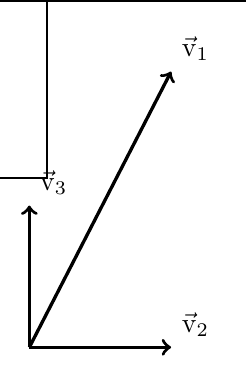
\begin{tikzpicture}
        \tkzInit[xmax=0.5,ymax=0.5,xstep=0.1,ystep=0.1]
        %\tkzAxeX[label=FancyBrand,above left=10pt]
        \tkzAxeX[label=FancyBrand, right]
        %\tkzAxeY[label=green,below right=30pt]
        \tkzAxeY[label=green,above]
        \tkzGrid
        \draw[very thick, ->] (0,0) -- (1.8,3.5) node[anchor=south west]{$\vec{\text{v}}_1$};
        \draw[very thick,latex-latex, ->] (0,0) -- (1.8,0) node[anchor=south west]{$\vec{\text{v}}_2$};
        \draw[very thick,latex-latex, ->] (0,0) -- (0, 1.8) node[anchor=south west]{$\vec{\text{v}}_3$};
    \end{tikzpicture}

    \caption{Two dimensional vector space model}
    \label{fig:vectorspacemodel}
\end{figure}


\subsubsection{Parametric and zone indices}
\label{sec:parametricandzoneindices}

% evtl. noch ausf\"uhren:
% - stop words (woerter die nicht gewertet werden z.b. ist, er war, ...)
% - Parametric and zones indices


\subsection{Rocchio's algorithm}
\label{sec:rocchio}
%%%%%%%%%%%%%%%%%%%%%%%%%%%%%%%%%%%%
\iffalse
Beschreibung des Rocchio algorithmus
\fi
%%%%%%%%%%%%%%%%%%%%%%%%%%%%%%%%%%%%
With section~\ref{sec:tfidf} and section~\ref{sec:vectorspacemodel} the requirements of Rocchio's algorithm have been described.\citep[p.~178]{manning:2009}
The next step is to specify the algorithm itself.
{\color{red} Kommt eigentlich aus information retrieval und hilft dabei items zu finden.
Bietet also vorschlaege zu einer suchanfrage, wobei die anfrage die bisher gewaehlten producte sind.}
Rocchio's relevance feedback algorithm is classified as content-based RS.\citep[p.~92]{lops:2011}
The algorithm tries to find a vector representing the user that is similiar to all item which are relevant to the user.
In addition the number of unrelevant item matching the vector should be minimal.\citep[p.~178-181]{manning:2009}
One of the algorithms charakteristics is the way feedback (as described in section~\ref{sec:feedback}) is treated.
Every time the user gives either positive or negative feedback, the algorithm will adapt the user vector to match the new criteria.\citep[p.~387-388]{pazzani:2007}
\\

When using Rocchio's algorithm for a recommender system one uses a user vector instead of a query vector as originally intended.
\begin{equation}
    \vec{\text{q}}_m =
        \alpha \cdot \vec{\text{q}}_0
        + \beta \cdot \frac{1}{|\text{D}_\text{r}|}\sum_{\vec{\text{d}}_j\in \text{D}_\text{r}} \vec{\text{d}}_j
        - \gamma \cdot \frac{1}{|\text{D}_\text{nr}|}\sum_{\vec{\text{d}}_j\in \text{D}_\text{nr}} \vec{\text{d}}_j
\end{equation}
$\vec{\text{q}}_0$ is the old vector representing the user before he gave feedback about one of the items.
The result $\vec{\text{q}}_m$ however is the modified vector describing the user after his most recent feedback has been considered.
For each calculation with Rocchio's algorithm $\vec{\text{q}}_0$ will always be the result $\vec{\text{q}}_m$ of the preceding calculation.\\
$\text{D}_\text{r}$ is a set of all relevant item vectors, while $\text{D}_\text{nr}$ represents a set of items that are unrelevant to the user.\\
$\alpha$, $\beta$ and $\gamma$ act as weights and can influence the importance of the old user vector, as well as of  the relevant and unrelevant documents.
The old user vector is weighted by $\alpha$.
The average of relevant documents is weighted by $\beta$ and $\gamma$ is responsible for unrelevant documents.
There are only positive values for weights allowed.
The lowest possible weight is 0.
A well established configuration for these weights is: $\alpha = 1$, $\beta = 0.75$ and $\gamma = 0.15$.
However if a RS only allows positive feedback, one can as well set $\gamma$ to 0.
\citep[p.~178-183]{manning:2009}



\section{Implementation}
Most of the theory behind RS and the methodology it depends on have already been introduced.
The implementation of a RS will be described in the following.
All examples have been written in a programming language called Python.
There is also some SQL code and some UML- and EER-diagrams in order to visualize the concept.
As database \gls{sqlite3} has been used.

\subsection{Content based RS in-depth}
\label{sec:implementation-contentbased}
The general framework for a content-based RS is shown in figure~\ref{fig:framework-contentbasedrs}.
There are three main components a content-based RS consists of.
\begin{itemize}
    \item \textbf{Content Analyzer}\hfill\\
        Since all items the RS has to work with are potentially unstructured, a pre-process is necessary to filter relevant information.
        This will be mainly done by IR-techniques.
        The Content Analyzer aims to bring all items in a form which can be used by its successional components.
        \citep[p.~75-77]{lops:2011}
    \item \textbf{Profile Learner}\hfill\\
        When the items are in a suitable form, the Profile Learner can construct a user profile.
        In case of Rocchio's algorithm this includes to distinguish all relevant items from non-relevant.
        Based on all items and the user's preferences the Profile Learner can build a user profile.
        Rocchio's algorithm uses a vector representing the users attitude towards different attributes of an item.
        In case of Rocchio, the user profile is a vector representing his attitude towards the different attributes an item may have.
        \citep[p.~75-77]{lops:2011}
    \item \textbf{Filtering Component}\hfill\\
        For each user profile the Filtering Component can find items which may match the users preferences.
        Depending on the method implemented the result can be a binary or continuous relevance judgment.
        The continuous relevance judgement is a list of ranked items.
        \citep[p.~75-77]{lops:2011}
        The RS implemented for this thesis uses k-nearest-neighbours classification.
        kNN results in a list of ranked items where $k$ best-ranked items will be suggested to the user.
\end{itemize}


\begin{figure}[h]
    \center
    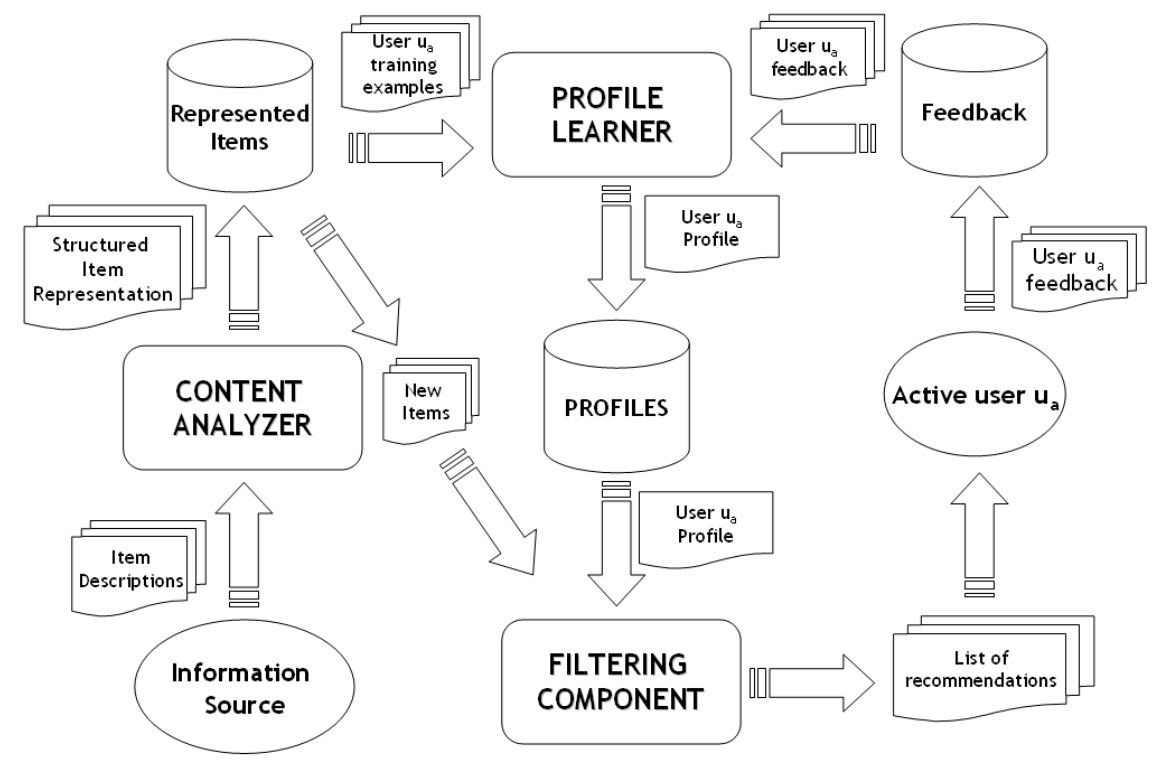
\includegraphics[scale=0.4,clip=true,trim=24px 0 15px 0]{inc/implementation/HighlevelContentBased}
    \caption{High level description of a content-based RS.\citep[p.~76]{lops:2011}}
    \label{fig:framework-contentbasedrs}
\end{figure}



\subsection{Content Analyzer}
\label{sec:content-analyzer}
\index{Content Analyzer}
%{Building the vectors}
%{Storage within the database}
For this project the data describing the products, offered by an online shop have been semi-structured.
It was a text file where each line described a product.
An example is given in listing~\ref{lst:product-data}.

\begin{lstlisting}[caption={Example product data},label={lst:product-data}
    ,keywordstyle=\color{black}
    ,commentstyle=\itshape\color{black}
    ,identifierstyle=\color{black}
    ,stringstyle=\color{black}
]
ImgURL Brand Product Price Shoulder_Width Model_Length Collar_Type Material
http://i1.ztat.net/large/4E/M2/1E/00/0K/11/4EM21E000-K11@4.jpg Emoi en Plus Bluse - dazzling blue 24,95 °(\euro{})° 50 cm 70 cm bei Gr°(\"{o}\ss{})°e 44 Rundhals 100% Polyester
http://i2.ztat.net/large/NA/52/1D/03/NA/11/NA521D03N-A11@3.jpg NAF NAF WENT - Bluse - ecru/noir 38,95 °(\euro{})° 55 cm bei Gr°(\"o{}\ss{})°e S Rundhals 64% Viskose, 22% Baumwolle, 10% Modal, 4% Polyamid
\end{lstlisting}

\noindent
Since the structure of the input was known, it was possible to filter out all relevant product information without using too fancy IR methods.
With regular expressions all relevant informations such as the product\_image-url, brand, product, price, collar type and material have been extracted and stored in a database.
Since a RS could theoretically handle any kind of item afar from products, a distinction has been made between documents in general and products.
The relation between a product and a document has been illustrated in figure~\ref{fig:ertermdocumentassignment}.
It is notable that all terms in a document are treated equally.
This means, that there are no parametric zones or such (section~\ref{sec:parametricandzoneindices}).
\begin{figure}[h]
    \center
    \includegraphics[scale=0.5]{inc/implementation/contentanalyzer/er_term_document_assignment}
    \caption{ER diagram of documents, products and associated terms}
    \label{fig:ertermdocumentassignment}
\end{figure}
Since the relation between \textit{Product} and \textit{Term} is N to N, an intermediate table is neccessary when transforming the ER-diagram into a relational model.
Therefore the table \textit{TermDocumentAssigner} will be introduced and the relational model will look as follows:

\begin{quote}
    \textbf{Document}{(\underline{document\_id})}\\
    \textbf{Product}{(\underline{document\_id[Document]}, image\_name)}\\
    \textbf{Term}{(\underline{term\_id}, name)}\\
    \textbf{TermDocumentAssigner}{(\underline{document\_id[Document], term\_id[Term]}, count)}\\
\end{quote}
\noindent
Since \textit{TermDocumentAssigner} will be very often used to query all terms of a document, it is useful to make an index on \textit{document\_id}.
Implicitly there will also be one on the combined primary key \textit{document\_id, term\_id}.
The tables, implemented by the RS build for this thesis, filled with example data may look as in table~\ref{tab:tablestermdocumentproduct}.
Table~\ref{tab:tablestermdocumentproduct} will serve as resource for terms and documents to illustrate subsequent examples.\\

\begin{table}

    \center

    % Document
    \rowcolors{1}{\dustRowFirst}{\dustRowSecond}
    \begin{tabular}{ l }
        \rowcolor{\dustRowHead}
        \textbf{Document}\\\hline
        document\_id\\\hline
        1\\
        2\\
        3\\
    \end{tabular}
    \quad
    % Product
    \rowcolors{1}{\dustRowFirst}{\dustRowSecond}
    \begin{tabular}{ l | l }
        \rowcolor{\dustRowHead}
        \multicolumn{2}{ c }{\textbf{Product}}\\\hline
        document\_id    & image\_name\\\hline
        1               & image\_1.png\\
        2               & image\_2.png\\
        3               & image\_3.png\\
    \end{tabular}

    ~\\

    %TermDocumentAssigner
    \rowcolors{1}{\dustRowFirst}{\dustRowSecond}
    \begin{tabular}{ l | l | l }
        \rowcolor{\dustRowHead}
        \multicolumn{3}{c}{\textbf{TermDocumentAssigner}}\\\hline
        document\_id    & term\_id  & count\\\hline
        1               & 1         & 1\\
        1               & 2         & 1\\
        1               & 4         & 1\\
        2               & 1         & 1\\
        2               & 3         & 1\\
        2               & 7         & 1\\
        3               & 4         & 1\\
        3               & 5         & 1\\
        3               & 6         & 1\\
    \end{tabular}
    \quad
    % Term
    \rowcolors{1}{\dustRowFirst}{\dustRowSecond}
    \begin{tabular}{ l | l }
        \rowcolor{\dustRowHead}
        \multicolumn{2}{ c }{\textbf{Term}}\\\hline
        term\_id        & name\\\hline
        1               & blouse\\
        2               & blue\\
        3               & polyester\\
        4               & cotton\\
        5               & green\\
        6               & trouser\\
        7               & white\\
    \end{tabular}
    \caption{Table layout defined by figure~\ref{fig:ertermdocumentassignment}}
    \label{tab:tablestermdocumentproduct}
\end{table}

\noindent
As already mentioned before, Rocchio's algorithm works best with tf-idf vectors.
Since the theory has been described in section~\ref{sec:tfidf}, the next big step is to show how vectors for this project have been built.
A short reminder: currently all products are described through their terms.\\

\noindent
In order to build tf-idf vectors, one also has to built term frequency, as well as inverse document frequency vectors - these are the preconditions.
Since these tasks are fairly similar, some design patterns help realizing them.
The \gls{abstract factory} pattern proofed to be very handy for this task.
For each necessary vector (tf, idf, tf-idf) one can build a vector creator which shares the design of the other vector creators.
Therefore the abstract class \textit{VectorCreator} has been introduced.
The \textit{VectorCreator} offers the abstract method \textit{\_get\_vector(document\_id:int):DocumentVector} which will be responsible for creating all vectors.
All inherited classes will implement the abstract method with a procedure to create an instance of \textit{DocumentVector}.

\paragraph{Term frequency vector}
\index{Term Frequency}
Every term frequency vector representing a document consists of the term frequency of all terms.
The current implementation uses the SQL query displayed in listing~\ref{lst:tf-query} for generating the tf vector.
The result of a query may look as follows (based on the tables shown in figure~\ref{fig:ertermdocumentassignment} and are displayed in table~\ref{tab:tf-query-result}.
\begin{table}
    \rowcolors{1}{\dustRowFirst}{\dustRowSecond}
    \begin{tabular}{ l|l|l || l|l|l || l|l|l }
        \rowcolor{\dustRowHead}
        \multicolumn{3}{c||}{\textbf{$\text{tf}_\text{document\_1}$}} &
        \multicolumn{3}{c||}{\textbf{$\text{tf}_\text{document\_2}$}} &
        \multicolumn{3}{ c }{\textbf{$\text{tf}_\text{document\_3}$}}\\\hline

        term\_id & name & value                          & term\_id & name  & value             & term\_id & name & value\\\hline
        1   & blouse    & 1                              & 1    & blouse    & 1                 & 1 & blouse  & 0\\
        2   & blue      & 1                              & 2    & blue      & 0                 & 2 & blue  & 0\\
        3   & polyester & 0                              & 3    & polyester & 1                 & 3 & polyester  & 0\\
        4   & cotton    & 1                              & 4    & cotton    & 0                 & 4 & cotton  & 1\\
        5   & green     & 0                              & 5    & green     & 0                 & 5 & green  & 1\\
        6   & trouser   & 0                              & 6    & trouser   & 0                 & 6 & trouser  & 1\\
        7   & white     & 0                              & 7    & white     & 1                 & 7 & white  & 0\\
    \end{tabular}
    \caption{Possible result of the query in listing~\ref{lst:tf-query}}
    \label{tab:tf-query-result}
\end{table}

\begin{lstlisting}[language=SQL,caption={SQL query for generating tf-vectors},label={lst:tf-query},float=h]
-- :document_id is a parameter given to the method
SELECT
    [t].[term_id]
    , [t].[name]
    , CASE WHEN  [a].[document_id] IS NULL
        THEN    0
        ELSE    [a].[count]
    END AS [value]
FROM
    [Term] AS [t]
    LEFT OUTER JOIN [TermDocumentAssigner] AS [a]
        ON  [t].[term_id] = [a].[term_id]
        AND [document_id] = :document_id
ORDER BY    [t].[term_id]
;
\end{lstlisting}

\noindent
The result of the query shown in listing~\ref{lst:tf-query} will finally be stored in the \textit{TermFrequencyVector} class derived from \textit{DocumentVector} (see figure~\ref{fig:uml-document-vectors}).

\paragraph{Document frequency vector}
\index{Document Frequency}
In contrast to the \textit{TermFrequencyVector} the \textit{DocumentFrequencyVector} does not resemble a single document, rather than the whole collection of documents.
Therefore the parameter \textit{document\_id} can be omitted.
But in order to sustain uniformity between all classes inheriting from \textit{VectorCreator} it will be carried along but set to a null value.
To make the source code more readable, the SQL code for querying the document-frequency values has been outsourced to a SQL-View as shown in listing~\ref{lst:df-view}.
This little tweak (that has no influence on speed) left the query for df-vectors as simple as shown in listing~\ref{lst:df-query}.
The result for the example is given in table~\ref{tab:df-query-result}.

\begin{lstlisting}[language=SQL,caption={SQL statement to create the \textit{DocumentFrequency}-view},label={lst:df-view},float=h]
CREATE VIEW IF NOT EXISTS [DocumentFrequency] AS
    SELECT
            [t].[term_id]
            , [t].[name]
            , CASE WHEN   [a].[count] IS NULL
                THEN        0
                ELSE        [a].[count]
            END AS [value]
    FROM
        [Term] as [t]
        LEFT OUTER JOIN
        (
            SELECT
                [term_id]
                , SUM([document_id]) AS [count]
            FROM
                [TermDocumentAssigner]
            GROUP BY
                [term_id]
        ) AS [a]
            ON [t].[term_id] = [a].[term_id]
    ORDER BY
        [t].[term_id]
;
\end{lstlisting}

\begin{lstlisting}[language=SQL,caption={SQL query for generating df-vectors},label={lst:df-query},float=h]
SELECT
    [term_id]
    , [name]
    , [value]
FROM
    [DocumentFrequency]
;
\end{lstlisting}

\begin{table}
    \center
    \rowcolors{1}{\dustRowFirst}{\dustRowSecond}
    \begin{tabular}{ l | l | l }
        \rowcolor{\dustRowHead}
        \multicolumn{3}{ c }{\textbf{df}}\\\hline
        term\_id    & name      & value\\\hline
        1           & blouse    & 2\\
        2           & blue      & 1\\
        3           & polyester & 1\\
        4           & cotton    & 2\\
        5           & green     & 1\\
        6           & trouser   & 1\\
        7           & white     & 1\\
    \end{tabular}
    \caption{Possible results of the query in figure~\ref{lst:df-query}}
    \label{tab:df-query-result}
\end{table}

\begin{figure}[h]
    \center
    \includegraphics[scale=0.4]{inc/implementation/contentanalyzer/uml_document_vectors}
    \caption{Document vectors}
    \label{fig:uml-document-vectors}
\end{figure}

\paragraph{Inverse document frequency vector}
\index{Inverse Document Frequency}
For building idf-vectors one can use df-vectors (and their source code) as basis.
The inverse document frequency is calculated by dividing the total count of documents in a collection through the document frequency of a term.
Another SQL-View called N-view will provide the number of documents, while the code for creating idf-vectors get outsourced into its own view once more.
Since the SQL implementation of \gls{sqlite3} does not offer a logarithm-function, one has to defined his very own.
Fortunately the standard python library for connecting to sqlite3-databases supports the creation of functions as shown in listing~\ref{lst:idf-view}.


\begin{lstlisting}[language=Python,caption={SQL-statement to create the InverseDocumentFrequency-view},label={lst:idf-view}]
def _create_log_function(self, conn):
    conn.create_function('log10', 1, InverseDocumentFrequencyVectorCreator.log_10)
    pass

def log_10(x):
    base = 10
    return math.log(x, base)
\end{lstlisting}
\begin{lstlisting}[language=SQL]
CREATE VIEW IF NOT EXISTS [InverseDocumentFrequency] AS
    SELECT
        [term_id]
        , [name]
        , log10
        (
            CAST ((SELECT [document_count] from [N]) AS REAL) / [df].[value]
        )
         AS [value]
    FROM
        [DocumentFrequency] AS [df]
    ORDER BY
        [term_id]
    ;
\end{lstlisting}


\begin{lstlisting}[language=SQL,caption={SQL-statement to create the N-view},label={lst:n-view},float=h]
CREATE VIEW IF NOT EXISTS [N] AS
    SELECT
        (SELECT COUNT(*) FROM [Document]) AS [document_count]
        , (SELECT COUNT(*) FROM [Term]) AS [term_count]
;
\end{lstlisting}


\begin{lstlisting}[language=SQL,caption={SQL-query for generating idf-vectors},label={fig:idf-query},float=h]
SELECT
    [term_id]
    , [name]
    , [value]
FROM
    [InverseDocumentFrequency]
;
\end{lstlisting}


\begin{table}
    \center
    \rowcolors{1}{\dustRowFirst}{\dustRowSecond}
    \begin{tabular}{ l | l | l }
        \rowcolor{\dustRowHead}
        \multicolumn{3}{ c }{\textbf{idf}}\\\hline
        term\_id    & name      & value\\\hline
        1           & blouse    & $\log_{10}(3/2) \approx 0.18$\\
        2           & blue      & $\log_{10}(3/1) \approx 0.48$\\
        3           & polyester & $\log_{10}(3/1) \approx 0.48$\\
        4           & cotton    & $\log_{10}(3/2) \approx 0.18$\\
        5           & green     & $\log_{10}(3/1) \approx 0.48$\\
        6           & trouser   & $\log_{10}(3/1) \approx 0.48$\\
        7           & white     & $\log_{10}(3/1) \approx 0.48$\\
    \end{tabular}
    \caption{Possible results of the query in figure~\ref{fig:idf-query}}
    \label{tab:idf-query-result}
\end{table}

\paragraph{Tf-idf vector}
\index{TfIdf}
Finally one can create tf-idf vectors which are the combination of tf- and idf-vectors (as explained in section~\ref{sec:tfidf}).
Since tf-idf is merely the multiplication of term frequency with the corresponding inverse document frequency, it's rather simple to calculate.
Listing~\ref{lst:tfidf-code} shows the creation of a \textit{TfIdfVector} in the method \textit{\_create\_vector()}, whereas the multiplication is in method \textit{\_get\_values()}.

\begin{lstlisting}[language=Python,caption={Python code for calculating tfidf-vectos on basis on tf- and idf-vectors},label={lst:tfidf-code},float=h]
class TfIdfVectorCreator(VectorCreator):

    def __init__(self, db_connection_str):
        super(TfIdfVectorCreator, self).__init__(db_connection_str)

        self._tf_creator = TermFrequencyVectorCreator(db_connection_str)
        self._idf_creator = InverseDocumentFrequencyVectorCreator(db_connection_str)
        pass

    def _create_vector(self, document_id):
        tf_vector = self._tf_creator.get_vector(document_id)
        idf_vector = self._idf_creator.get_vector(document_id)

        tfidf_vector = TfIdfVector()

        for triple in self._get_values(tf_vector, idf_vector):
            tfidf_vector.add_to_vector(triple)

        return tfidf_vector

    def _get_values(self, tfv, idfv):
        ingredients = zip(tfv.term_id, tfv.description, tfv.values, idfv.values)

        for (tf_tid, tf_desc, tf_val, idf_val) in ingredients:
            yield (tf_tid, tf_desc, tf_val * idf_val)
            pass
        pass
\end{lstlisting}

\begin{table}
    \rowcolors{1}{\dustRowFirst}{\dustRowSecond}
    \begin{tabular}{ l|l|l || l|l|l || l|l|l }
        \rowcolor{\dustRowHead}
        \multicolumn{3}{c||}{\textbf{$\text{tf-idf}_\text{document\_1}$}} &
        \multicolumn{3}{c||}{\textbf{$\text{tf-idf}_\text{document\_2}$}} &
        \multicolumn{3}{ c }{\textbf{$\text{tf-idf}_\text{document\_3}$}}\\\hline

        term\_id & name & value             & term\_id & name & value           & term\_id & name & value\\\hline
        1   & blouse    & $\approx 0.18$    & 1    & blouse   & $\approx 0.18$  & 1 & blouse      & 0\\
        2   & blue      & $\approx 0.48$    & 2    & blue     & 0               & 2 & blue        & 0\\
        3   & polyester & 0                 & 3    & polyester& $\approx 0.48$  & 3 & polyester   & 0\\
        4   & cotton    & $\approx 0.18$    & 4    & cotton   & 0               & 4 & cotton      & $\approx 0.18$\\
        5   & green     & 0                 & 5    & green    & 0               & 5 & green       & $\approx 0.48$\\
        6   & trouser   & 0                 & 6    & trouser  & 0               & 6 & trouser     & $\approx 0.48$\\
        7   & white     & 0                 & 7    & white    & $\approx 0.48$  & 7 & white       & 0\\
    \end{tabular}
    \caption{Possible result of the function in figure~\ref{lst:tfidf-code}}
    \label{tab:tfidf-query-result}
\end{table}


With the vectors built, the main task of the content analyzer is done.
However there is still one more enhancement one can implement to make the repetitive creation of vectors faster.
Through dynamic (for details see section~\ref{sec:dynamic-programming}) programming we can easily "re-create" vectors we already used once.
Since it proves useful, if all inheriting classes of \textit{VectorCreator} can use dynamic programming without explicitly implementing it, one can implement the \textit{VectorCreator} as proxy (explained in sectin~\ref{sec:proxy}).
As a result the \textit{VectorCreator} gets another method called \textit{get\_vector(document\_id:int)} to which the same rules apply as to \textit{\_create\_vector(document\_id:int)}.
The buffering of \textit{DocumentVectors} can now be implemented in \textit{get\_vector(document\_id:int)} and all inheriting classes will also posses caching capabilities.
The code for dynamic programming is shown in listing~\ref{lst:dynamic-programming}.\\
In order to get a picture of all important vectors and their creation, a UML-diagram has been included (figure~\ref{fig:uml-vectorssimple}).

\begin{lstlisting}[language=Python,caption={Dynamic programming},label={lst:dynamic-programming},float=h]
class VectorCreator(object):

    # ... omitted unnecessary code

    def get_vector(self, document_id=None):
        if document_id is not None and not isinstance(document_id, int):
            raise TypeError('document_id must either be an integer or None')
        if not document_id in self._cache:
            vector = self._create_vector(document_id)
            if vector.document_id is None:
                vector.document_id = document_id
            self._cache[document_id] = vector
        return self._cache[document_id]}

    def _create_vector(self, document_id):
        # ... creating vector
\end{lstlisting}


\begin{figure}[h]
    \center
    \includegraphics[scale=0.33,angle=90]{inc/implementation/contentanalyzer/uml_vectors_simple}
    \caption{Abstract and concrete vector fabric}
    \label{fig:uml-vectorssimple}
\end{figure}

\FloatBarrier

\subsection{Profile Learner}
%{Rocchio algorithm}
%{Relevance feedback}
With the products in a database and being capable to form them into vectors, the next step is to implement the profile learner.
As already mentioned the algorithm of choice is Rocchio's algorithm (introduced in section~\ref{sec:rocchio}).
It creates a user vector that gets refined every time the user gives feedback about his preferences.
Therefore a new table that holds the user vector is necessary.
Furthermore one has to store the users feedback towards some of the documents.
The er-diagram in figure~\ref{fig:er_user_table} shows the layout which has been implemented.\\
Each user is identified by an unique id (\textit{user\_id}) and optionally by a also unique name (\textit{name}).
Any user can specify his preferences by marking some documents as relevant.
This will be further explained when discussing the possibilities of user feedback.
{\color{red}TODO}
Because the algorithm can work with any of the stored items, it rather works on \textit{Documents}, than on \textit{Products}.
For each of the terms which define a document the user has a "value" that defines his attitude towards the term.
The more similar the users value of a term $t$ is with a $\text{tf-idf}_t$ value of a document, the more likely he can can make use of the document/product.
The users position towards a term is stored within the relation between the user and the corresponding term.

% user vector creator and uservector
\begin{figure}[h]
    \center
    \includegraphics[scale=0.5]{inc/implementation/profilelearner/er_user_table}
    \caption{ER diagram of user and his related entities}
    \label{fig:er_user_table}
\end{figure}

\noindent
When forming the er diagram in figure~\ref{fig:er_user_table} into a relational schema the result will look like below.
Whereas the user is represented by \textit{User}, the N-to-N relation between \textit{User} and \textit{Document} will be solved by a new table \textit{UserPreference} and the relationship between \textit{User} and \textit{Term} with a attribute becomes \textit{UserVector}.
\begin{quote}
    \textbf{User}($\underline{\text{user\_id}}$, name)\\
    \textbf{UserPreference}($\underline{\text{user\_id[userManagement]},\text{document\_id[Document]}}$)\\
    \textbf{UserVector}($\underline{\text{user\_id[UserManagement], term\_id[Term]}}$, value)\\
\end{quote}

% user vector
\begin{figure}[h]
    \center
    \includegraphics[scale=0.3]{inc/implementation/profilelearner/uml_vector_user}
    \caption{UML diagram describing UserVector and UserVectorCreator}
    \label{fig:uml_vector_user}
\end{figure}

\begin{lstlisting}[language=SQL,caption={SQL query for creating a user vector},label={lst:user-vector-query},float=h]
SELECT
    [t].[term_id]
    , [t].[name]
    , [uv].[value]
FROM
    [Term] AS [t]
    JOIN [UserVector] AS [uv]
        ON [t].[term_id] = [uv].[term_id]
WHERE
    [uv].[user_id] = :user_id
ORDER BY
    [t].[term_id]
;
\end{lstlisting}

\begin{table}
    \rowcolors{1}{\dustRowFirst}{\dustRowSecond}
    \begin{tabular}{ l | l }
        \rowcolor{\dustRowHead}
        \multicolumn{2}{c}{\textbf{User}}\\\hline
        user\_id    & name \\\hline
        1           & user\_test\\
    \end{tabular}
    \quad
    \rowcolors{1}{\dustRowFirst}{\dustRowSecond}
    \begin{tabular}{ l | l }
        \rowcolor{\dustRowHead}
        \multicolumn{2}{c}{UserPreference}\\\hline
        user\_id    & document\_id\\\hline
        1           & 2\\
    \end{tabular}
    \quad
    \rowcolors{1}{\dustRowFirst}{\dustRowSecond}
    \begin{tabular}{ l | l | l }
        \rowcolor{\dustRowHead}
        \multicolumn{3}{c}{UserVector}\\\hline
        user\_id    & term\_id  & value\\\hline
        1           & 1         & 0\\
        1           & 2         & 0\\
        1           & 3         & 0\\
        1           & 4         & 0\\
        1           & 5         & 0\\
        1           & 6         & 0\\
        1           & 7         & 0\\
    \end{tabular}
    \caption{User table and dependencies filled with example values}
    \label{tab:user}
\end{table}

\noindent
Listing~\ref{lst:rocchio} finally displays the implementation of Rocchio's algorithm.
Based on the example set up in section~\ref{sec:content-analyzer}, there is an example how the algorithms changes user vectors.\\
Parameter \textit{q\_0} of function \textit{calculate()} is the current vector that represents the user.\\
Rocchio's algorithm will create a new vector that refines and replaces the current one.
\textit{list\_d\_related} is a list of related documents (the terminology is derived from information retrieval).
Any document that the user marked as preferences counts as relevant.\\
A list of all irrelevant documents will be passed via \textit{list\_d\_unrelated}.\\
It is possible to either use pre-defined weightings for the variables $\alpha$, $\beta$, or $\gamma$, represented by "a", "b" and "c".
But of course the user of the library can also define his very own weights by passing a triple as fourth parameter to the function \textit{calculate}.
When no weights are passed explicitly, the function will call \textit{default\_weights()} in order to gain the pre-set default values.
Based on the weights the result for refined user vector will vary greatly.\\
The return value \textit{q\_m} finally is the updated user vector that must replace the vector stored in table \textit{UserVector}.
When this is done, one has successfully used Rocchio's algorithm to adopt a user vector to the users feedback.
An example is given below.

\begin{lstlisting}[language=Python,caption={Implementation of Rocchio's algorithm},label={lst:rocchio},float=h]
def default_weights():
    a = 1
    b = 0.85
    c = 0.15
    return (a, b, c)

def calculate(q_0, list_d_related, list_d_unrelated, weights=default_weights()):
    a, b, c = weights

    def calculate_a():
        return q_0.scalar_multiplication( a )

    def calculate_b():
        if len(list_d_related) > 0:
            return (
                    sum(list_d_related)
                    .scalar_multiplication(1/len(list_d_related))
                ).scalar_multiplication(b )
        return null_vector()

    def calculate_c():
        if len(list_d_unrelated) > 0:
            return (
                    sum(list_d_unrelated)
                    .scalar_multiplication(1/len(list_d_unrelated))
                ).scalar_multiplication(c)
        return null_vector()

    def null_vector():
        empty = q_0.scalar_multiplication(0)
        return empty
        
    q_m = calculate_a() + calculate_b() - calculate_c()
    return q_m
\end{lstlisting}

\noindent
Assuming that the user also likes document 1 and therefore gives the RS feedback about document 1, Rocchio's algorithm would work as shown in the equation below (based on the values in table~\ref{tab:user} and \ref{tab:idf-query-result}).
By comparing $\text{q}_0$ with the modified vector $\text{q}_\text{m}$ one can see in which way the vector has changed (the initial vector $\text{q}_0$ has been set to this value by default).
\begin{align*}
    \alpha &= 1;\quad \beta = 0.85;\quad \gamma = 0.15\\
    \text{q}_0 &= (0, 0, 0, 0, 0, 0, 0)^T \\
    \text{l}_\text{dr} &= \{(0.18, 0.48, 0, 0.18, 0, 0, 0)^T, (0.18, 0, 0.48, 0, 0, 0, 0, 0.48)^T\}\\
    \text{l}_\text{dnr} &= \{(0, 0, 0, 0, 0.18, 0.48, 0.48, 0)^T\}\\
    \text{q}_\text{m} &=
        \alpha \cdot \text{q}_0
        + \beta \cdot \frac{1}{|\text{l}_\text{dr}|}\sum_{\text{d}_\text{j}\in\text{l}_\text{dr}}\vec{\text{d}}_\text{j}
        - \gamma \cdot \frac{1}{|\text{l}_\text{dnr}|}\sum_{\text{d}_\text{j}\in\text{l}_\text{dnr}}\vec{\text{d}}_\text{j}\\
    &= 1 \cdot (0, 0, 0, 0, 0, 0, 0)^T\\
        &\quad+ 0.85 \cdot \frac{1}{2} \cdot \big((0.18, 0.48, 0, 0.18, 0, 0, 0)^T+(0.18, 0, 0.48, 0, 0, 0, 0, 0.48)^T \big)\\
        &\quad- 0.15 \cdot \frac{1}{1} \cdot(0, 0, 0, 0, 0.18, 0.48, 0.48, 0)^T\\
    &= (0, 0, 0, 0, 0, 0, 0)^T\\
        &\quad+(0.153, 0.204, 0.204, 0.0765, 0, 0, 0.204)^T\\
        &\quad-(0, 0, 0, 0.027, 0.072, 0.072, 0)^T\\
    &= \underline{\underline{
            (0.153, 0.204, 0.204, 0.0495, -0.072, -0.072, 0.204)^T
        }}
\end{align*}

\FloatBarrier

\subsection{Filtering Component}
%%%%%%%%%%%%%%%%%%%%%%%%%%
%k nearest neighbours
% manning 297, 290 (euclidean distance)
%%%%%%%%%%%%%%%%%%%%%%%%%%
\index{filtering component}
\label{sec:filtering-component}
{\color{red}\tiny Discuss euclidean and hamming distance}
As filtering component $k$ nearest neighbours (kNN) has been implemented.
One of its advantages is, that it does not require any training or whatsoever.\citep[p.~290]{manning:2009}
kNN will return a list of the $k$ closest vectors around a given centroid.
Therefore $k$ can be interpreted as a parameter.
When the value for $k$ is already determined (for instance $k=3$), than one can also speak of 3NN.\citep[p.~297-298]{manning:2009}
To measure distance between two vectors the algorithm relies on the Euclideans distance, as is has been suggested by \citeauthor{manning:2009}.\citep[p.~292]{manning:2009}
For comparision other ways for calculating the distance have also been implemented - namely the Hamming distance.
When using kNN it is recommended to choose a value $k > 1$, since otherwise it is deemed as not robust.
It's also better to choose an odd value for $k$.\\
An implementation of $k$NN with exchangeable distance function is displayed in listing~\ref{lst:knn}.

\begin{lstlisting}[language=Python,caption={kNN and distance methods},label={lst:knn},float=h]
def hamming_distance(v1, v2):
    return v1.hamming_distance(v2)

def euclidean_distance(v1, v2):
    return v1.euclidean_distance(v2)

default_distance = euclidean_distance

def k_nearest_neighbours(k, vector_origin, vectors, distance_function=default_distance):
    distances = [(distance_function(vector_origin, v), v) for v in vectors]
    ratings = distances
    ratings.sort()  # sorts ascending by distance, then by DocumentVector
    return [(r, v) for (r, v) in ratings[:k] ]

class DocumentVector(object):

    # ... omitted uneccesary code

    def hamming_distance(self, other):
        distance = 0
        for val1, val2 in zip(self.values, other.values):
            if not val1 == val2:
                distance += 1
        return distance

    def euclidean_distance(self, other):
        t = sum(
            ((v1 - v2) ** 2  for v1, v2 in zip(self.values, other.values))
        )
        d = math.sqrt(t)
        return d
\end{lstlisting}

The \textit{k\_nearest\_neighbours} function awaits a $k$ as first parameter, specifying the size of the list to return.
As second parameter the function gets a vector which suits as fixpoint for calculating the distances called \textit{vector\_origin}.
\textit{vectors} are all vectors whose distance shall be measured.
As an optional argument \textit{k\_nearest\_neighbours} awaits a function for calculating the distance.
Per default, the function is \textit{euclidean\_distance} which calculates the euclidean distance between two vectors.

When using this $k$NN with the euclidean distance function on the data of the example, the results will look as in the table~\ref{tab:knn-result}.
As parameter $k$ 2 has been chosen.



\begin{table}
    \center
    \rowcolors{1}{\dustRowFirst}{\dustRowSecond}
    \begin{tabular}{ l | l | l }
        \rowcolor{\dustRowHead}
        rank    & distance              & document\_id\\\hline
        1       & 0.43305340317332686   & 1\\
        2       & 0.45553841769931985   & 2\\
        %3       & 0.8801677396951105    & 3\\
    \end{tabular}
    \caption{Possible $k$NN result for $k=2$}
    \label{tab:knn-result}
\end{table}

\FloatBarrier

\subsection{Recommender library}
"Recommender library" labels the whole programming code which has been written for this thesis to a build programming library capable of creating item recommendations based on Rocchio's algorithm as declared in the milestones (figure~\ref{fig:softwaremilestones}).
In short it will be called "recommender.lib".
Since the previous sections already solved the goals defined by the milestones up to the library, this section describes recommender.lib's usage.

Following tasks are managed by recommender.lib:
\begin{itemize}
    \item Adding and removing products which can be recommended
    \item Creating, updating and removing users
    \item Making recommendations based on a user profile
\end{itemize}

\paragraph{Initialize recommender.lib}
In order to use recommender.lib on has to connect it to a database.
All database-tables required by recommender.lib will be created automatically when needed.
As main component \textit{DatabaseManager} delegates all tasks to other classes and gives access to them.
\begin{lstlisting}[language=Python,caption={Startup of recommender.lib},label={lst:recommenderlib-startup}]
import recommender
databasepath = "./database/recommender.sqlite3"
manager = recommender.DatabaseManager(databasepath)
\end{lstlisting}

\paragraph{Insert products}
With \textit{DatabaseManager} one can retrieve \textit{ProductManager} who is responsible for inserting and deleting products.
Afterwards a product can be added.
A product is no more than a collection of terms which describe it.
A term can be added by \textit{Product.add\_term()} with an optional second parameter describing its frequency.
If the parameter is omitted, the term's frequency will be set to 1.
\textit{Product} as derived class of \textit{Document} has an image\_name as special tweak which is used to store the file path of an image which represents the product.
\begin{lstlisting}[language=Python,caption={Insertion of products},label={lst:recommenderlib-product-insertion}]
product_manager = manager.get_product_manager()
p = recommender.product.Product()
p.image_name = 'image_01.png'
p.add_term('white')
p.add_term('blouse', 1)
product_manager.add_document(p)
\end{lstlisting}

\paragraph{Get product vectors}
With products added one can easily get their vectors (for example their \textit{tf-idf}-vectors).
In order to do so, one calls \textit{ProductVectorManager.get\_tfidf\_vector()} with the corresponding document\_id.
\textit{ProductVectorManager} also offers methods for creating \textit{tf}-, \textit{df}- and \textit{idf}-vectors.
When new products have inserted afterwards one has to delete all cached items of the \textit{ProductVectorManager} by calling \textit{ProductVectorManager.flush()}.
\begin{lstlisting}[language=Python,caption={\textit{tf-idf} vector of a product},label={lst:recommenderlib-product-vector}]
pvm = manager.get_product_vector_manager()
tfidf_vector = pvm.get_tfidf_vector(1)
print(tfidf_vector.values)  # prints: (0.0, 0.0)
\end{lstlisting}

\paragraph{Add users}
As next step a user will be created with \textit{UserVectorManager}.
Any user requires a user name which identifies him.
Recommender.lib however gives any user a unique id.
Methods working on users either require a \textit{user\_name} or \textit{user\_id}.
When a user is freshly created his vector will consist of numeric null.
\begin{lstlisting}[language=Python,caption={Add user},label={lst:recommenderlib-user-add}]
uvm = manager.get_user_vector_manager()
user_name = 'test_user'
uvm.create_user(user_name)
user_id = uvm.get_user_id_for_name(user_name)
user_vector = uvm.get_user_vector_for_id(user_id)
print(user_vector.values)   # prints: (0.0, 0.0)
\end{lstlisting}

\paragraph{Execute Rocchio's algorithm}
At the time there are both products available and users created one can start collecting user feedback.
Assuming that the user gives positive feedback towards the currently single product available the following listing will execute it.
The product will be marked as relevant and Rocchio's algorithm applied.
\begin{lstlisting}[language=Python,caption={Execute Rocchio's algorithm},label={lst:recommenderlib-rocchio}]
product_id = 1
uvm.set_user_preference(user_id, product_id, True)

relevant = uvm.get_relevant_document_vector_list(user_id)
non_relevant = uvm.get_non_relevant_document_vector_list(user_id)

updated_user_vector = recommender.rocchio.calculate(user_vector, relevant, non_relevant)
uvm.update_user_vector(user_id, updated_user_vector)
\end{lstlisting}

\paragraph{Finding recommendations}
Finally one can search for products which are similar to the user's vector.
This can be done by using \textit{k-nearest-neighbours} on the list of products and a user.
As a result a list with $k$ entries will be returned.
This list represents all recommendations.
Since kNN requires a distance-function for finding the nearest neighbours one can pass either a custom one, or use one of the pre-defined ones.
Currently supported are euclidean and hamming distance.
Because this kNN-implementation returns a combination of the distance and product-vectors, the vectors may have to be extracted.
\begin{lstlisting}[language=Python,caption={Retrieving recommendations},label={lst:recommenderlib-knn}]
distance_function = recommender.vector.arithmetic.euclidean_distance
k = 3
list_of_products = pvm.get_all_vectors()
meta_recommendations = recommender.vector.arithmetic.k_nearest_neighbours(
    k,
    updated_user_vector,
    list_of_products,
    distance_function
)
recommendations = [ vector for (distance, vector) in meta_recommendations ]
\end{lstlisting}

%Umfang und Aufgaben der Lib erkl\"aren.
\subsection{Web-API}
In order to operate the library from different programming languages except from Python a \gls{web api} has been implemented.
This API offers the most frequently function-calls a program using recommender.lib will require.
The online-shop introduced in section~\ref{sec:online-shop} has been written in \gls{javascript} calling the \gls{web api}.
Any request received by the web api through \gls{http} will result in a result containing a \gls{json} document.
An exhaustive list of all functions offered by the \gls{web api} and their return value is available in the appendix~\ref{sec:web-api}.


\subsection{Online shop}
As already mentioned in previous sections it is not the goal to implement a fully functional online shop as one may know it from Amazon.com or similiar vendors.
Instead this one focuses on offering products, collecting feedback from the user and finally generating recommendations which will be presented to the user.

\subsubsection{General look and feel}
The key functionality of given an overview of items and recommendations is being displayed in figure~\ref{fig:onlineshop-overview}.
While random products are displayed in the left column, possible recommendations will be displayed in the right colum which is highlighted in light green.
As soon as one clicks on one of the items displayed a product view will be opened where most of the information about the selected product will be available.
The product view is responsible for receiving and interpreting the users feedback and will be further explained in section~\ref{sec:onlineshop-feedback}.

\begin{figure}[h]
    \center
    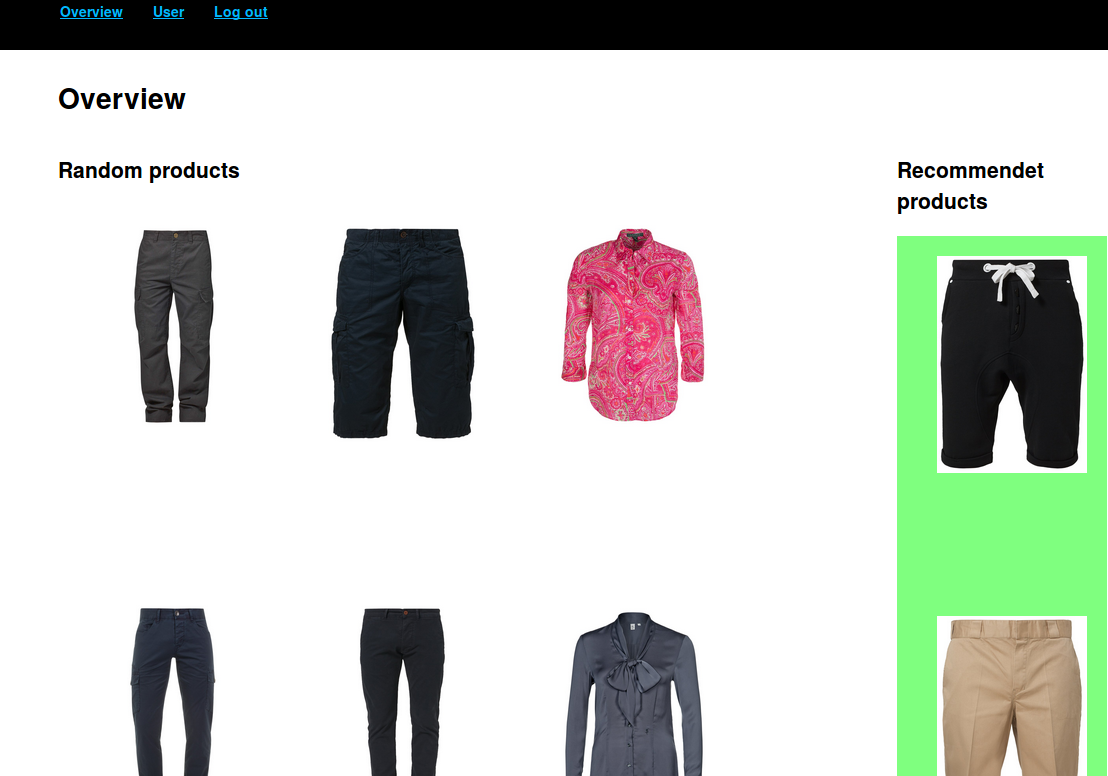
\includegraphics[scale=0.3]{inc/implementation/onlineshop/recommender_onlineshop_overview}
    \caption{Online shop overview}
    \label{fig:onlineshop-overview}
\end{figure}

\subsubsection{Feedback}
\label{sec:onlineshop-feedback}
Both implicit and explicit feedback as introduced in section~\ref{sec:feedback} have been implemented.
Even thought the initial task was to implement a RS that utilizes implicit feedback, explicit has been implemented as well to compare both methods.
There are three different ways of collecting feedback used by the online shop.
\begin{itemize}
    \item \textbf{Implicit}\hfill\\
        Whenever the user selects an item from the online-shops overview this will be interpreted as positive feedback towards the item.
    \item \textbf{Implicit timed}\hfill\\
        Instead of interpreting every item the user examines as explicit indicator for sympathy towards the product it will be measured how long the user views the product.
        It is assumed, that if the user still views the product after a pre-determined period of time he might be interessted in this particular item.
    \item \textbf{Explicit binary rating}\\
        The product-view will be equiped with a binary rating component which enables the user to explicitely like or dislike an item.
        This allows the user to remove items from the list of liked items which is not possible for the prior listed implicit methods since the user couldn't actively dislike an item.
\end{itemize}

Since implicit feedback do not require any interaction with a user there is no user interface with which a user can interact.
For explicit feedback however the user has been given the opportunity to give a binary rating about a item whether he likes it or not.
A snippet of the user interace for explict rating is shown in figure~\ref{fig:onlineshop-explicit-rating}.

\begin{figure}[h]
    \center
    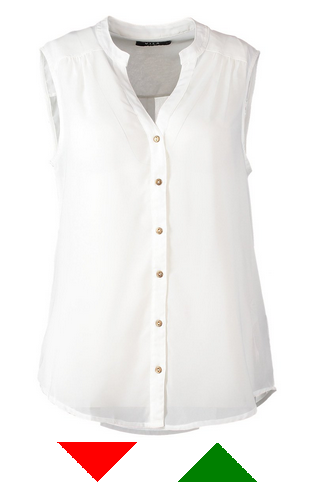
\includegraphics[scale=0.3]{inc/implementation/onlineshop/recommender-onlineshop-binary_rating}
    \caption{Binary rating of an item}
    \label{fig:onlineshop-explicit-rating}
\end{figure}


\subsubsection{Differences to real onine shops}
Even thought there are major differences between the implemented online shop and

%tracking through cookies

\FloatBarrier




\section{Outlook}

%%%%%%%%%%%%%%%%%%%%%%%%%%%%%%
Was kann man noch alles mit recommender dingern machen?
- im physischem geschaeft
Microsoft baut machine learning in sein Betriebssystem ein
%%%%%%%%%%%%%%%%%%%%%%%%%%%%%%
How can the rocchio algorithm be implemented in a ”real” (online-)shop?


% the license
%\section{License}
All code in this thesis written by the author will be published under a MIT-license.
\\

\begin{quote}
Copyright (c) 2015 \dustAuthor

Permission is hereby granted, free of charge, to any person obtaining a copy of this software and associated documentation files (the "Software"), to deal in the Software without restriction, including without limitation the rights to use, copy, modify, merge, publish, distribute, sublicense, and/or sell copies of the Software, and to permit persons to whom the Software is furnished to do so, subject to the following conditions:

The above copyright notice and this permission notice shall be included in all copies or substantial portions of the Software.

THE SOFTWARE IS PROVIDED "AS IS", WITHOUT WARRANTY OF ANY KIND, EXPRESS OR IMPLIED, INCLUDING BUT NOT LIMITED TO THE WARRANTIES OF MERCHANTABILITY, FITNESS FOR A PARTICULAR PURPOSE AND NONINFRINGEMENT. IN NO EVENT SHALL THE AUTHORS OR COPYRIGHT HOLDERS BE LIABLE FOR ANY CLAIM, DAMAGES OR OTHER LIABILITY, WHETHER IN AN ACTION OF CONTRACT, TORT OR OTHERWISE, ARISING FROM, OUT OF OR IN CONNECTION WITH THE SOFTWARE OR THE USE OR OTHER DEALINGS IN THE SOFTWARE.
\end{quote}


% affidavit/sworn declaration



\section*{Eidesstattliche Erklärung}

%Ich erkläre hiermit an Eides Statt, dass ich die vorliegende Arbeit selbständig und ohne fremde Hilfe angefertigt und alle Abschnitte, die wörtlich oder annähernd wörtlich aus einer Veröffentlichung entnommen sind, als solche kenntlich gemacht habe, ferner, dass die Arbeit noch nicht veröffentlicht und auch keiner Prüfungsbehörde vorgelegt worden ist.
%\\[4cm]

Ich versichere, dass ich die Arbeit ohne fremde Hilfe und ohne Benutzung anderer als der angegebenen Quellen angefertigt habe und dass die Arbeit in gleicher oder \"ahnlicher Form noch keiner anderen Pr\"ufungsbeh\"orde vorgelegen hat und von dieser als Teil einer Pr\"ufungsleistung angemonnen wurde.
Alle Ausf\"uhrungen, die w\"ortlich oder sinngem\"a\ss\;\"ubernommen wurden, sind als solche gekennzeichnet.
\\[4cm]


\noindent
%Fürth, den \displaydate{date}~$\underset{\text{\myAuthor}}{\underline{\hspace{5cm}}}$
Fürth, den \today~$\underset{\text{\dustAuthor}}{\underline{\hspace{5cm}}}$


% print glossary
%\makeglossaries

% Abbildungsverzeichnis
\listoffigures

%bibliograpy
\bibliographystyle{abbrvnat}
\bibliography{thesis}

\end{document}
